\documentclass{scrartcl}

\usepackage{fk-media}
\usetikzlibrary{lindenmayersystems}

\pgfdeclarelindenmayersystem{Koch curve}{\rule{F -> F-F++F-F}}

\begin{document}
  \begin{table}
    \centering
    \begin{tabular}{ccc}
      \toprule
        Item & Price \\
      \midrule
      Apple & 5 \\
      Car & 100 \\
      Butterfly & 50 \\
      \bottomrule
    \end{tabular}
    \caption{A basic table}
  \end{table}
  \begin{figure}
    \centering
    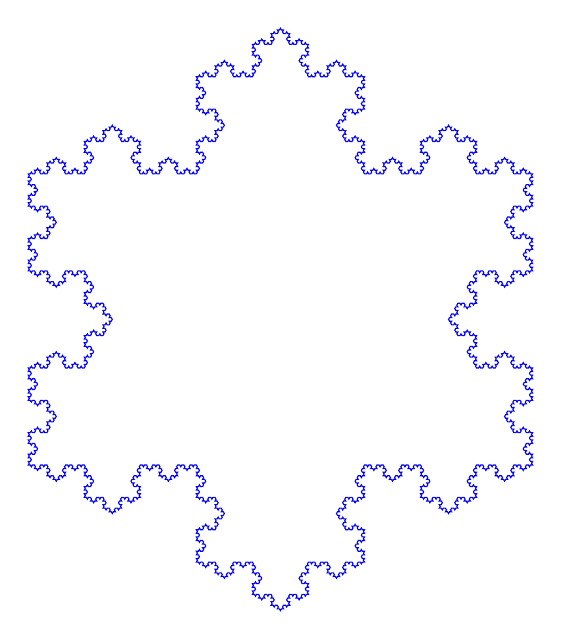
\begin{tikzpicture}
      \draw[blue] [l-system={Koch curve, step=0.75pt, angle=60, axiom=F++F++F, order=5}] lindenmayer system -- cycle;
    \end{tikzpicture}
    \caption{A TikZ drawing}
  \end{figure}
\end{document}
